\documentclass[10pt]{beamer}

\usetheme{m}
\renewcommand{\mthemetitleformat}{\scshape\MakeLowercase}
\usepackage{booktabs}
\usepackage[scale=2]{ccicons}
\usepackage{cancel}
\usepgfplotslibrary{dateplot}
\usepackage{pdfpages}
\usepackage{graphicx}
\usepackage{enumitem}
\setlist[description]{font=\normalfont\itshape}
\setlist[itemize]{font=\normalfont\itshape\textbullet\space}

\setlength{\arrayrulewidth}{0.2mm}
\setlength{\tabcolsep}{12pt}
\renewcommand{\arraystretch}{1.5}

\title{
    Abjad:\protect\\ 
    an open-source software system\protect\\ 
    for formalized score control
}
\subtitle{Introductory Workshop}
\author{
    Trevor Ba\v{c}a \inst{1} \and 
    Josiah Wolf Oberholtzer \inst{1} \and 
    Jeffrey Trevi\~{n}o \inst{2}
}
\institute[shortinst]{
    \inst{1}Department of Music, Harvard University \and 
    \inst{2} Department of Music, Colorado College
}
\date[CFP 2003]{
    Study Day on Computer Simulation of Musical Creativity\protect\\ 
    (Saturday 27 June 2015)
}

\begin{document}

\maketitle

\begin{frame}
    \frametitle{Table of Contents}
    \setbeamertemplate{section in toc}[sections numbered]
    \tableofcontents[hideallsubsections]
\end{frame}

\begin{frame}{Introduction}
The Abjad API for Formalized Score Control extends the Python programming
language with an open-source, object-oriented model of common-practice music
notation that enables composers to build scores through the aggregation of
elemental notation objects.
\end{frame}

\section{\emph{In media res}: Rhythm-makers}

\section{Abjad?}

\begin{frame}{Object model}
    \begin{center}
        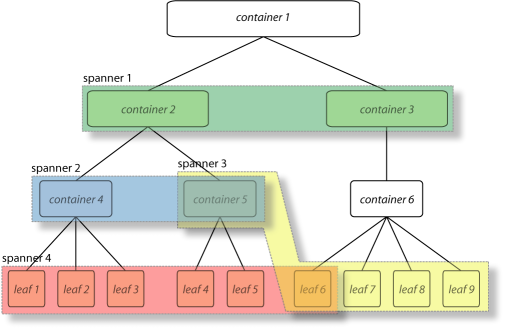
\includegraphics[scale=0.6]{container-spanner.png}
    \end{center}
\end{frame}

\begin{frame}{Code statistics}
    \begin{itemize}
        \item 496 public classes
        \item 387 public functions
        \item 186,963 lines of code
        \item 9399 unit tests
        \item 10190 documentation tests
    \end{itemize}
\end{frame}

\begin{frame}{History}
    \begin{itemize}
        \item C into Finale via MIDI (1997)
        \item Mathematica into Sibelius via MIDI (2001)
        \item Mathematica into SCORE (2003)
        \item Mathematica into LilyPond (2004)
        \item Python into Adobe Illustrator (2004)
        \item Python into LilyPond (2005)
        \item Max/MSP into MS Access into Adobe Illustrator (2008)\footnote{
            An attempt by Josiah before discovering Abjad.
            } 
        \item Public release on GoogleCode (2008)
        \item Migration to GitHub (2011)
        \item Abjad 2.16 released (2015)
    \end{itemize}
\end{frame}

\begin{frame}{Stack}
    \begin{table}
        \caption{Abjad Software Stack}
        \begin{tabular}{ |c|c|c|c|c| }
            \hline
            \multicolumn{5}{|c|}{\textbf{Python}} \\
            \hline
            \multicolumn{5}{|c|}{\textbf{Abjad}} \\
            \hline
            \xcancel{\textbf{Score}} & \textbf{LilyPond} & \textbf{Steinberg?} & ... & ... \\
            \hline
        \end{tabular}
    \end{table}
\end{frame}

\section{Score Applications}

\begin{frame}{Josiah's music}
    \begin{description}
        \item[2015] \textbf{Invisible Cities (iii): Ersilia} \\
            for chamber orchestra
        \item[2015] \textbf{Invisible Cities (ii): Armilla} \\
            for viola duet
        \item[2014] \textbf{Invisible Cities (i): Zaira} \\
            for eight players
        \item[2014] \textbf{Plague Water} \\
            for bari sax, e-guitar, piano and percussion
        \item[2011] \textbf{Aurora} \\
            for string orchestra
        \item[2010] \textbf{Lagartija} \\
            for mixed quartet
    \end{description}
\end{frame}

\begin{frame}{Jeff's music}
\begin{description}
\item[2015]\textbf{On the Behavior of Climbing Plants} \\ for chamber orchestra
\item[2013]\textbf{The World All Around} \\ for Eb clarinet, prepared piano, and harp
\item[2013]\textbf{+/-} \\ for twenty french horns
\item[2013]\textbf{Enfilade, Moses All, and Future Calendars} \\ for carillon
\item[2011]\textbf{Being Pollen} \\ for solo percussion

\end{description}
\end{frame}

\begin{frame}{Trevor's music}
\end{frame}

\begin{frame}{Other composers}
\begin{description}
\item Mike Solomon
\item Fredrik Wallberg
\item Oscar Dub
\item ???
\end{description}
\end{frame}

\section{Non-score Applications}

\begin{frame}{IPython}
\end{frame}

\begin{frame}{SASHA}
\end{frame}

\begin{frame}{nCoda}
\end{frame}

\section{Conclusion}

\begin{frame}{Online Presence}

\textbf{Documentation} \\
http://projectabjad.org

\vfill{}

\textbf{GitHub Repository} \\
http://github.com/Abjad/abjad

\vfill{}

\textbf{User Mailing List} \\
http://groups.google.com/group/abjad-user

\end{frame}

\begin{frame}{Personal Contacts}
    \begin{columns}[t,onlytextwidth]
        \column{.5\textwidth}
        \textbf{Trevor Ba\v{c}a}
        \begin{itemize}
            \item trevor.baca@gmail.com
            \item trevorbaca.com
            \item github.com/trevorbaca
        \end{itemize}
        \column{.5\textwidth}
        \textbf{Jeffrey Trevi\~{n}o}
        \begin{itemize}
            \item jeffrey.trevino@gmail.com
            \item jeffreytrevino.com
            \item github.com/jefftrevino
        \end{itemize}
    \end{columns}
    \vspace{\baselineskip}
    \textbf{Josiah Wolf Oberholtzer}
    \begin{itemize}
        \item josiah.oberholtzer@gmail.com
        \item josiahwolfoberholtzer.com
        \item github.com/josiah-wolf-oberholtzer
    \end{itemize}
\end{frame}

\end{document}